\chapter[Pulse collecting device and pulse database]{\uppercase{Pulse
collecting device and pulse database}}
\label{chap:two}

The acquisition of wrist pulse plays an crucial role in the
objectification, standardization and automation of pulse diagnosis.
Generally speaking, the quality of pulse signals obtained in the stage
has much to do with the subsequent sections, to some extent, deciding
the analysis performance of overall system. In the pulse
objectification history, pulse analytical instruments took on the
responsibility to transform human oscillation signal to visualized
images or figures easy to observe. And the designing of transducer
takes up the most part of electropulsograph development. The paper 
uses pulse collecting apparatus based on the fusion of pressure
sensors and photoelectric sensors to obtain pulse data. Then it
displays the way to collect pulse information. At last, the
construction of pulse database is explained in the paper. 

\section{Pulse collecting system}
So far, The pulse sensor has a wide range of types,
and uneven performances, which can be commonly divided into four
categories by the principle of work. One is the pressure sensor, by
detecting the pressure fluctuation at the position of radial artery
and describe the pulse image; Second is photoelectric sensor, by 
perceiving the change of vascular volume to describe the pulse information;
Third is the microphone, a sensor based on acoustics theories, in a
way to pick up the vibration caused by the pulse, i.e.
``listening'' to the signal; The last one is the ultrasonic Doppler technique.
\par 1. Pressure sensor
\par In the pressure sensor category, the piezoresistance pressure transducer
is the most widely used, which perceives the vibration of pulse on the
attribution that the resistivity changes along with the deformation
degree of medium. The attribution render the limitation that the
strain gauge must be attached on the test piece or the elastic
element in test. In the case, the performance of adhesive will
directly affect the operating feature of strain gauges (e.g.
creep deformation, mechanical lag, insulation resistance, sensitivity,
nonlinearity) and the extent of changes of these features over time or
temperature. Consequently, it restricts the accuracy, linearity and the scope
of application to the strain pressure sensor.
\par 2. Photoelectric sensor 
\par Here is its detection principle: Fluctuations in blood flow
cause the change of blood volume per unit, and the amount of blood
volume decides the portion of the light absorbed by blood. So when the
light is cast on the tissue, the amount of light reflected varies with
the fluctuation of blood flow. Finally the photoelectric transducer
converts the optical signal into electrical signal to reflect the change
of pulse waveform. 

The photoelectric transducer implements photoelectric
isolation, reducing interference to the next level of analog
circuit. Hence, it has high anti-jamming capacity, high sensitivity, 
good linearity and frequency response characteristic. Due to
insufficient acknowledgement to the internal connection between the vascular volume
and pulse information, only two indicators oxygen and pulse rate
can not meet the need for other blood stream arguments. 
\par 3. Microphone
\par The research in recent years shows wrist pulse signal is
naturally a kind of infrasonic wave, a vibration transmitting over the
special medium radial artery. Binghe Wang et al. adopted indirect
coupling (i.e. non-contact) extraction method to acquire the spectrum
characteristic of PingMai and XuanMai. An air column is set up to couple the
acoustic wave produced by vibration of wrist pulse.~\cite{B.1998}
\par 4. Ultrasonic Doppler technique
\par Besides the pressure information, arterial pulse includes lumen volume, blood flow
rate, three-dimensional vascular motion and other information. The
solo pressure factor hardly reflects the indicator of each component
in pulse. With the development of medical ultrasonic imaging technology, 
the application of ultrasound Doppler technique keeps its pace on the
objectification of pulse image. DongYu Zhang et al. extracted pulse
signal in the form of envelope line from the ultrasonic
image.~\cite{zhang2008wavelet} 

Although microphone and ultrasonic Doppler technique could receive
more information, the principle betrays the traditional pressing type
sphygmotechny. So the both hardly reflect the features of pulse
correctly.

The pulse collecting apparatus adopted in the subject is jointly
developed by Harbin Institution of Technology and HongKong PolyTechnic
University. See Figure~\ref{fig:device}. In the light of a better simulation of fingertips-touch
pulse diagnosis than the other sensors and its more convenient way of
fixation and pressurization, the pressure sensor is preferred. For
comparison purpose, photoelectric sensors are also built in the probe.
Therefore, the system contains 9 photoelectric transducers and one
pressure sensor in each position, totally 30 sensors. The upper screws
are used to increase pressure. The probe is shown in
Figure~\ref{fig:probe}. 

The pressure sensors and photoelectric transducers convert pulse
signal to analog electric signal. Then the signal is optimized in the
signal processing module, transformed in A/D converter and saved in
computer via USB line. 
\begin{figure}[htbp]
    \centering
    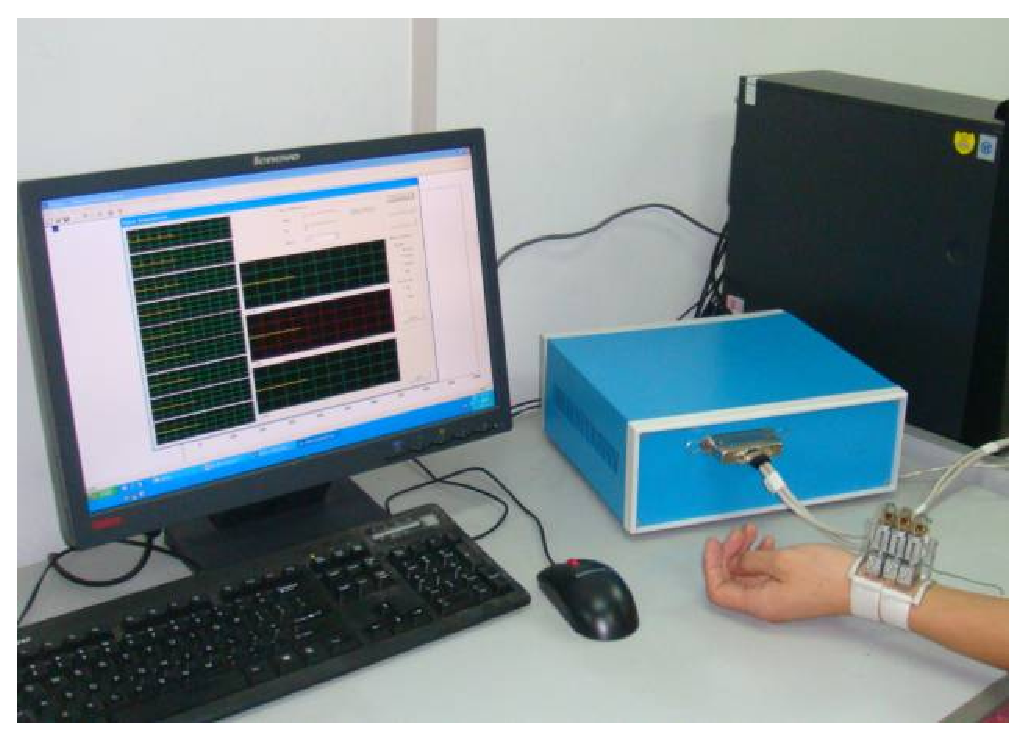
\includegraphics[width=0.6\textwidth]{device}
    \caption{Pulse collecting system}
    \label{fig:device}
\end{figure}
\begin{figure}[htbp]
    \centering
    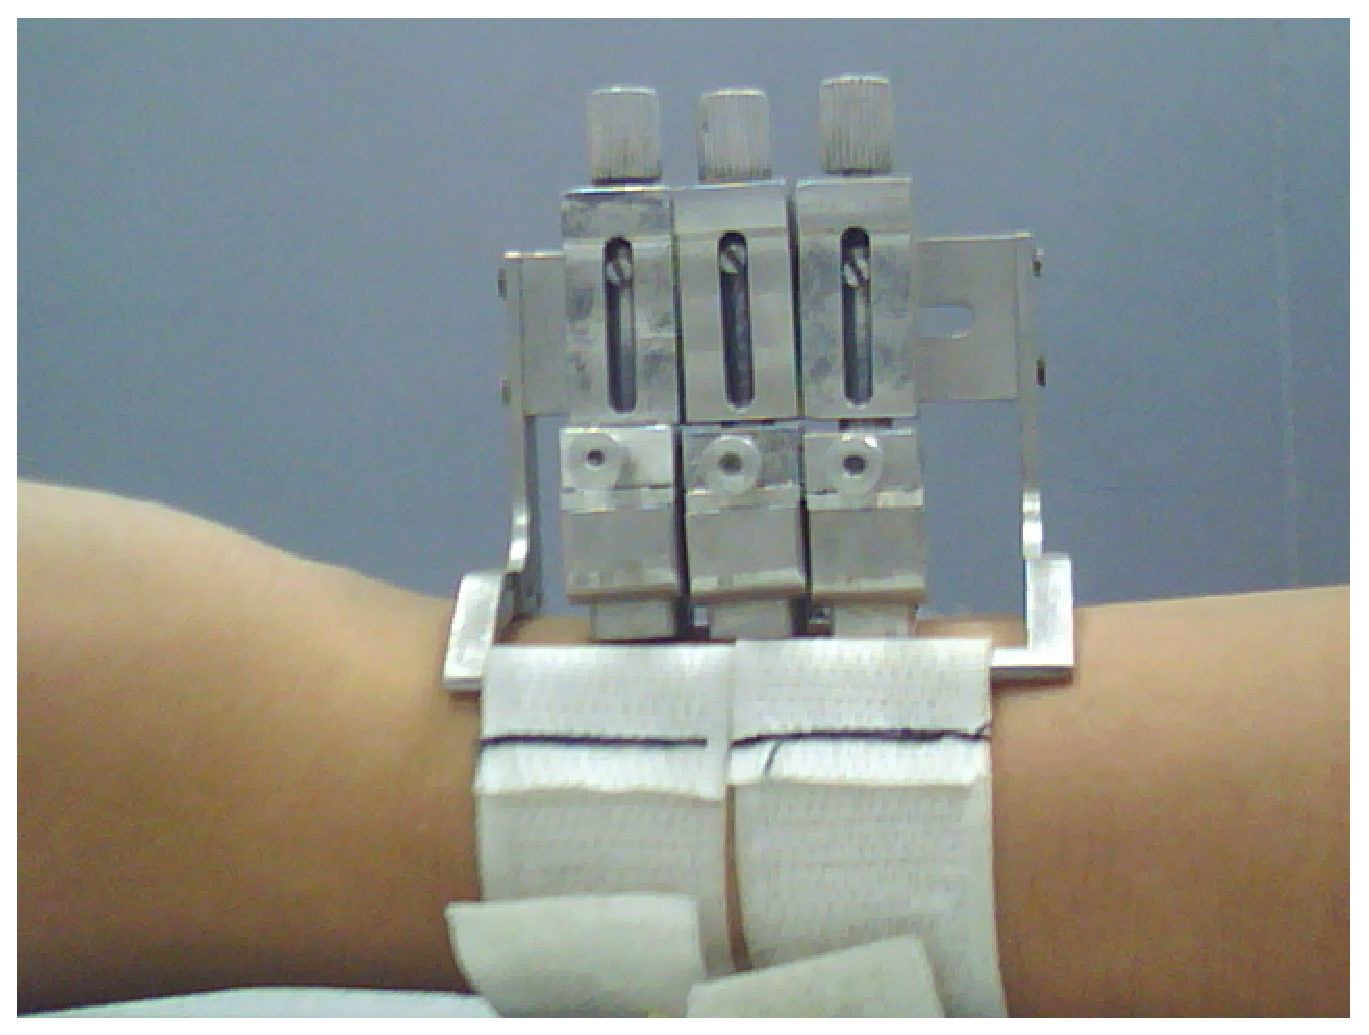
\includegraphics[width=0.6\textwidth]{probe}
    \caption{Probe head: fusion of photoelectric sensors and pressure sensors}
    \label{fig:probe}
\end{figure}
The biological signal of human body is a kind of continuous time
signal, which is difficult to process in computer. Therefore, the
pulse collecting apparatus fulfills this task and transmits
digital signals to computer. However, the overall process may loss a
certain amount of information. In other words, the digitalized signal
losses part of information during conversion. That is what 
The theorem describes two processes in signal processing: a sampling
process, in which a continuous time signal is converted to a discrete
time signal, and a reconstruction process, in which the original
continuous signal is recovered from the discrete time signal.
According to Nyquist theorem, the sampling frequency must be at least 
twice the highest frequency contained in the signal, or in
mathematical terms:
\begin{equation}
    f_s \geq f_e
    \label{eq:nyquist}
\end{equation}
where $f_s$ is the sampling frequency (how often samples are taken per
unit of time or space), and $f_e$ is the highest frequency contained
in the signal. So our device sets default frequency as 500Hz so as to
capture more details.  

The system is redesigned based on the model of first generation pulse
detecting system made by Harbin Institution of Technology. See
Figure~\ref{fig:1stgen}. Compared with the first generation system,
the new system has the following advantages:
\begin{enumerate}[(1)]
    \item Acquire more information. The pulse length and pulse width
        could be obtained. 
    \item Plug-and-play. The system reaps the benefits of USB 2.0
        which makes devices easy to use.
    \item Locate function. The photoelectric sensor array helps
        practitioners quickly locate the right position of radial artery. 
    \item Modularized design. Six independent modules, i.e. sensors, analog
        circuits, digital circuits, firmware, driver and application,
        reduce the probability to break down and let improvement and
        maintenance easier.
\end{enumerate}
\begin{figure}[htpb]
    \begin{center}
        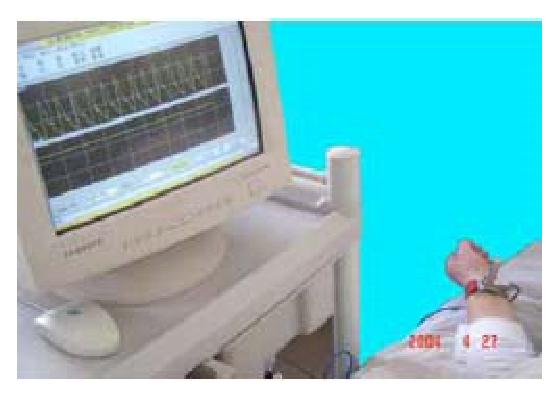
\includegraphics[width=0.8\textwidth]{1stgen}
    \end{center}
    \caption{The first generation of pulse detecting system developed
    by Harbin Institution of Technology}
    \label{fig:1stgen}
\end{figure}

In spite of the advantages described above, the system still exposed
a few deficiencies listed as follows: 
\begin{enumerate}[(1)]
    \item Poor durability. In pulse collection period, four or five
        continuous working seems common. Unfortunately, some sensors
        malfunction as sudden with the result that signals on those channels
        remain null. So the incompleteness of signal information brings
        trouble to the further analysis. 
    \item Unstable. The pressure value often drifts unexpectedly
        during collection. Normally it wanders around 200g, but
        sometimes it jump to 7000g, that is impossible. Probably the
        bug occurs in the strain gauge. In addition, it is hard to
        keep the same of pressure values on three positions. 
    \item Bad operability. During actual manipulation, even skilled
        practitioners fail to ensure all three positions detect
        signals. The three probe heads relates each other that
        adjustment on one probe head may displace others. 
\end{enumerate}

\section{The collection of wrist pulse}
It is worth to explain the detail of pulse collecting process for the
sake of understanding the simulation of pulse diagnosis via
automated apparatus. 
\par 1. Record personal information 
\par As is known to all, lung, spleen, liver and
kidney are all basic entrails as well as heart to maintain the
body functions. The diversity of morphological structures and
physiological characteristics to these entrails generates the
corresponding the five internal organs. Besides, in view of the tight
relationship of entrails with heart, pulse, Qi in TCM, blood, the
interaction and coordination among them has influence on pulse shape.
Moreover, the wrist pulse may vary due to the change of mental health
even though the physical organs work well. Hence, before the
collection, the biological indexes (e.g. gender, age, height, weight)
are also needed as a reference approach. A person information
management dialog is designed in view of convenience
shown as Figure~\ref{fig:dialog}.
\begin{figure}[htpb]
    \begin{center}
        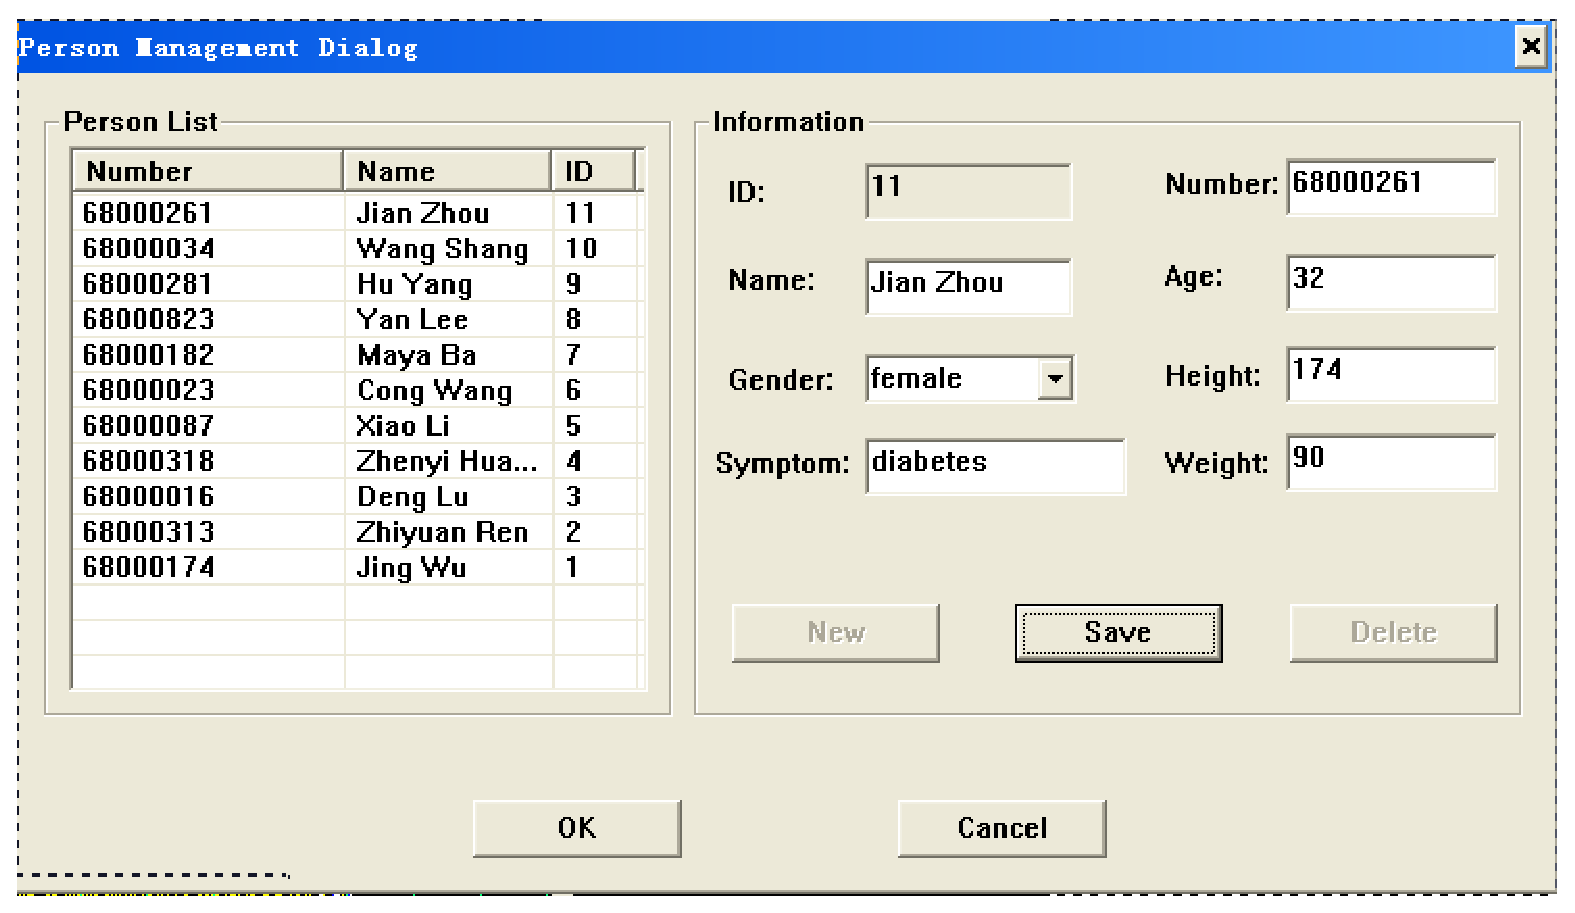
\includegraphics[width=0.9\textwidth]{dialog}
    \end{center}
    \caption{Person management interface}
    \label{fig:dialog}
\end{figure}
\par 2. Hand selection
\par In TCM pulse diagnosis, the practitioners usually use three fingertips (Index,
Middle and Ring fingers) to touch the left hand of patient and feel
the pulse fluctuation on three positions, i.e. `Cun', `Guan' and
`Chi'. Hence, in order to best simulation, the left hand is selected
in this experiment.
\par 3. Wrist pulse detecting process 
\par  The signal collection process includes usually three
steps. 
\begin{enumerate}[(1)]
    \item Find a rough location in the wrist. The
    practitioners use the three fingertips mentioned above to feel the
    proper position of the wrist (the experiment adopts the left
    hand) to place the probe. Generally speaking, the practitioner
    should ensure the probe detect signals on each position. 
    \item Fine tune and observation. 
        Take the Guan part as example. There are nine photoelectric
        sensors in the part. If the intensity of signals detected
        on one side are much stronger than the other side, then 
        it indicates that the sensor should be slightly fine-tuned
        towards the weak side. It also works to other two positions.
    \item Repeat the foregoing steps until signals from three points
        are observable, including pressure sensors and photoelectric
        sensors. See Figure~\ref{fig:interface}.
    \item Adjust pressure value. The paper imitates the process of 
        pulse diagnosis to feel the intensity of radial artery signals 
        in different pressure values. By manually twisting the screw
        of probe, pressure value to the radial artery could change. 
        Figure~\ref{fig:pressure} shows the intensity divergence of pulse
        signals under 130g, 200g, 250g pressures. The amplitude
        increases by \hl{1.8} when
        the pressure increases from \hl{130} to \hl{200g}
        while the amplitude yet decreases by about \hl{0.5} when the
        pressure value increases from \hl{200g} to \hl{250}.
        Therefore, the pressure value is considered as the best value to
        show the pulse obtained.
    \item Record 2-3 records. Each record should last at least 10
        seconds. During the sampling period, no laughing and talking
        is allowed. 
\end{enumerate}
\begin{figure}[htpb]
    \begin{center}
        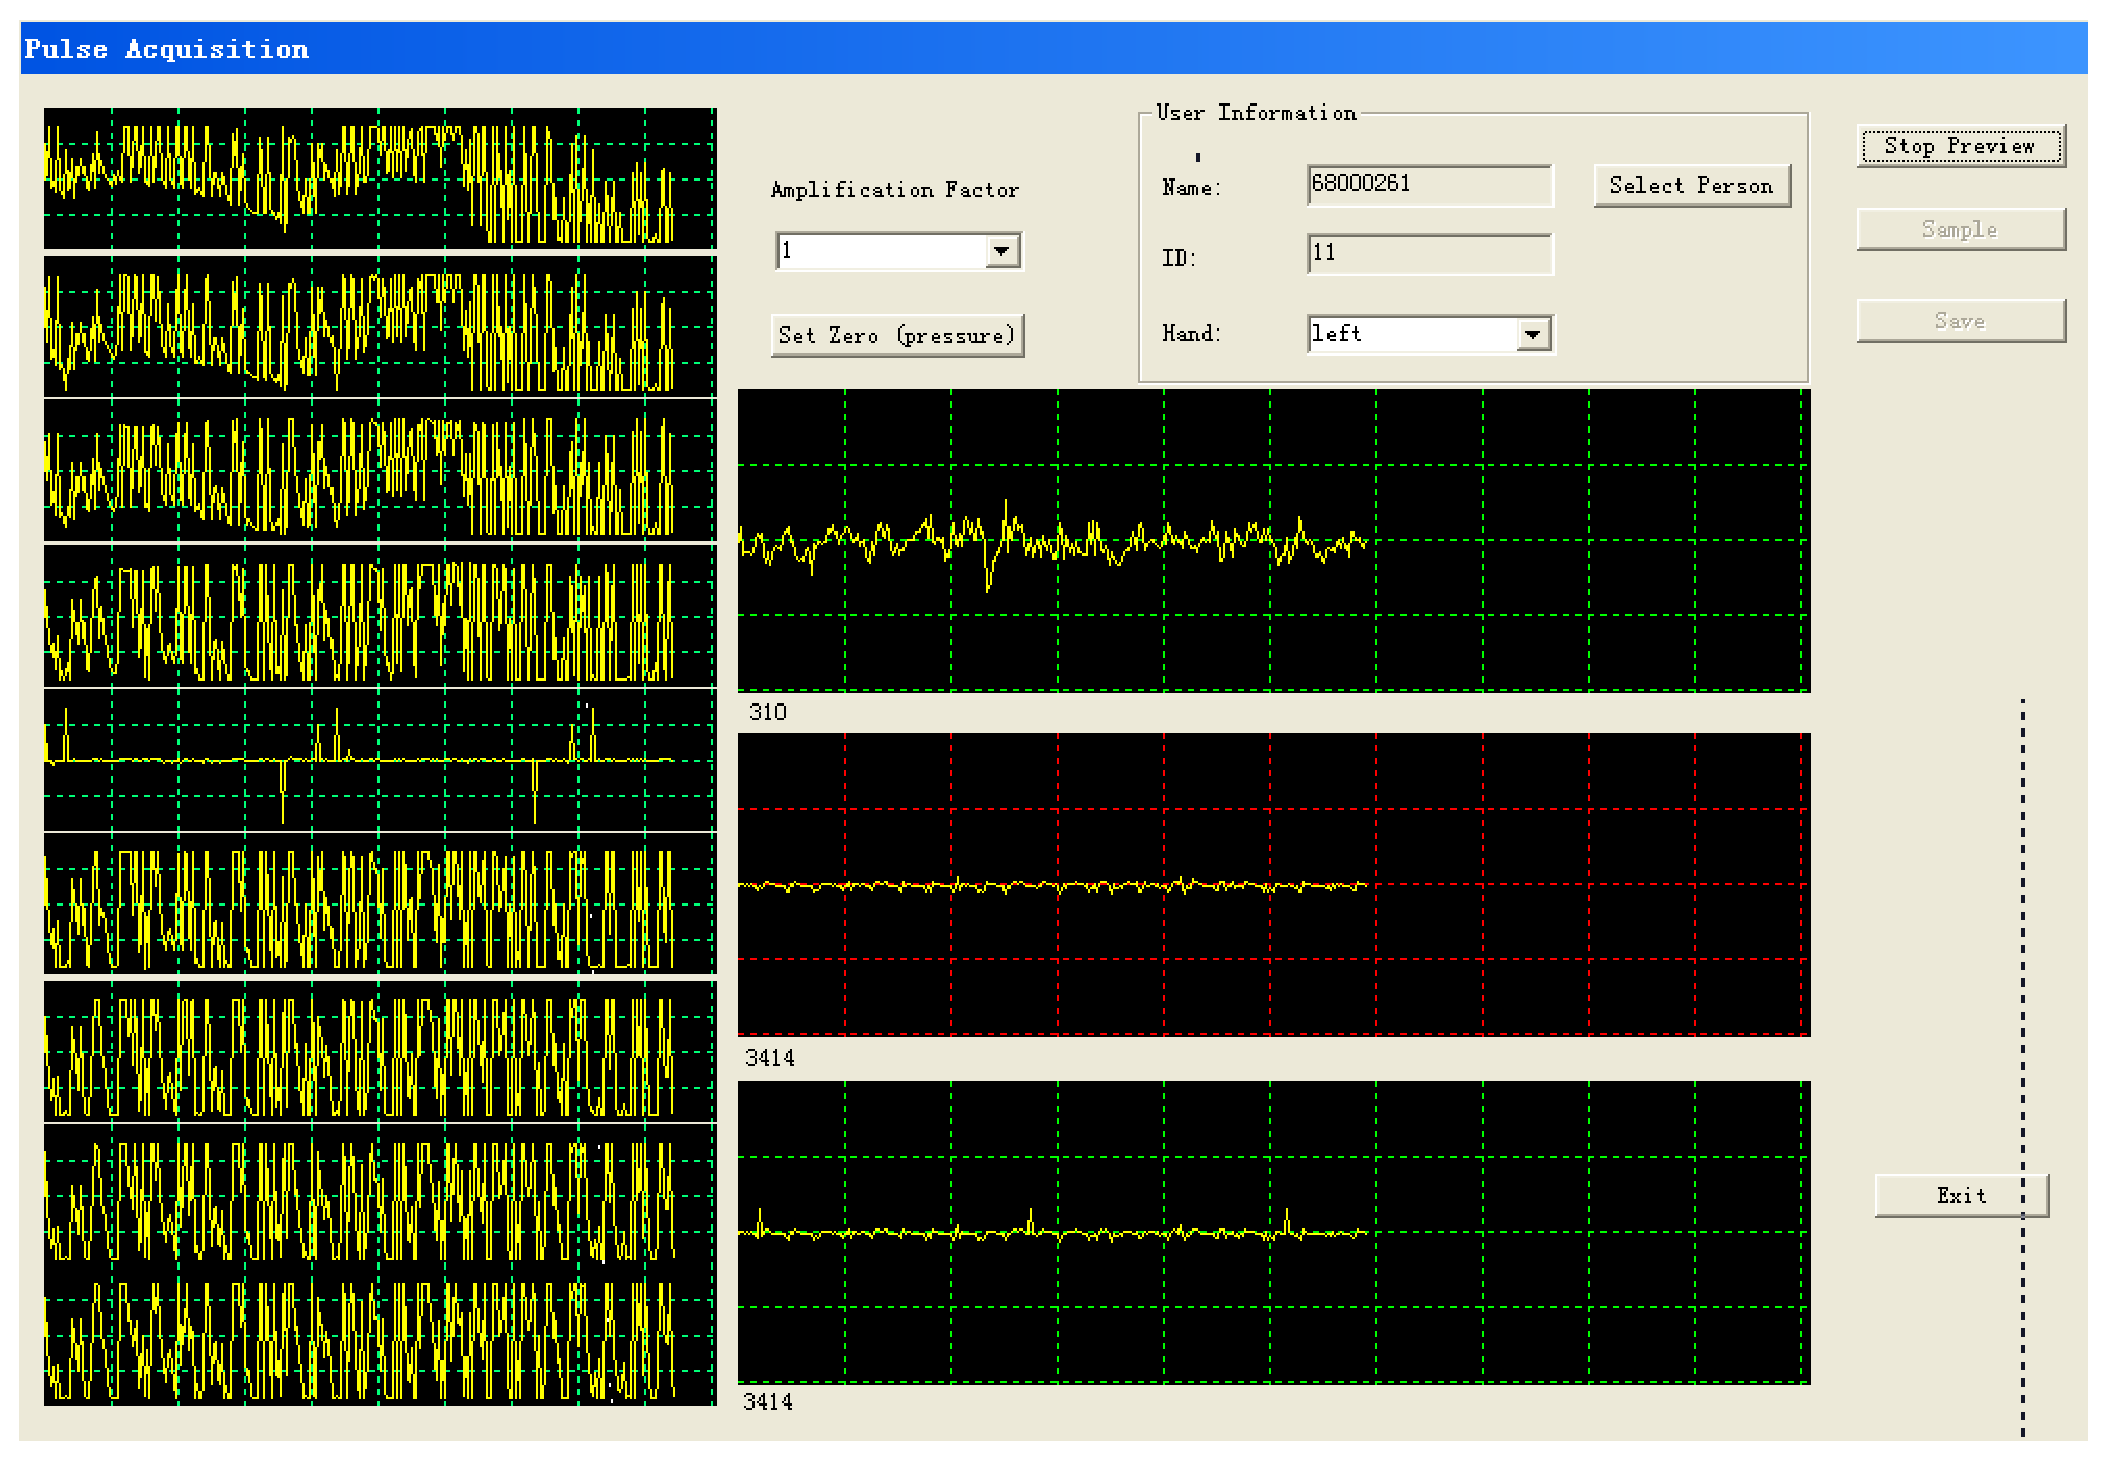
\includegraphics[width=0.7\textwidth]{interface}
    \end{center}
    \caption{Main interface for pulse collection}
    \label{fig:interface}
\end{figure}

\begin{figure}[htbp]
    \centering
    \subfloat[Pulse signal when the pressure is
    130]{\label{fig:130g}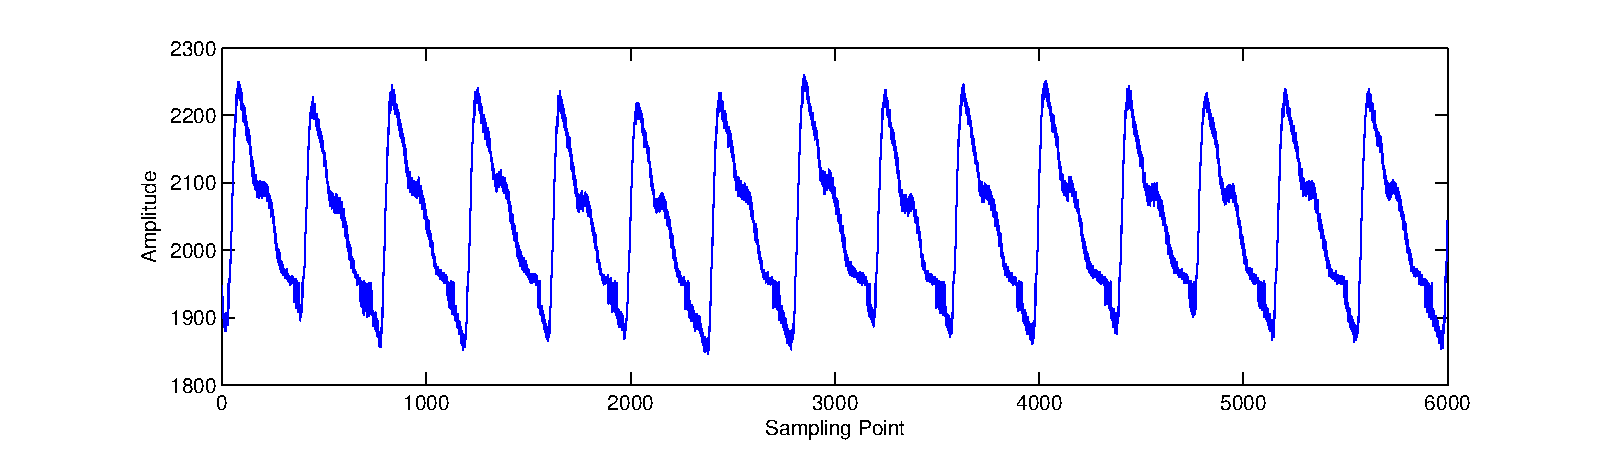
\includegraphics[width=0.7\textwidth]{130g}}\\
    \subfloat[Pulse signal when the pressure is
    200g]{\label{fig:200g}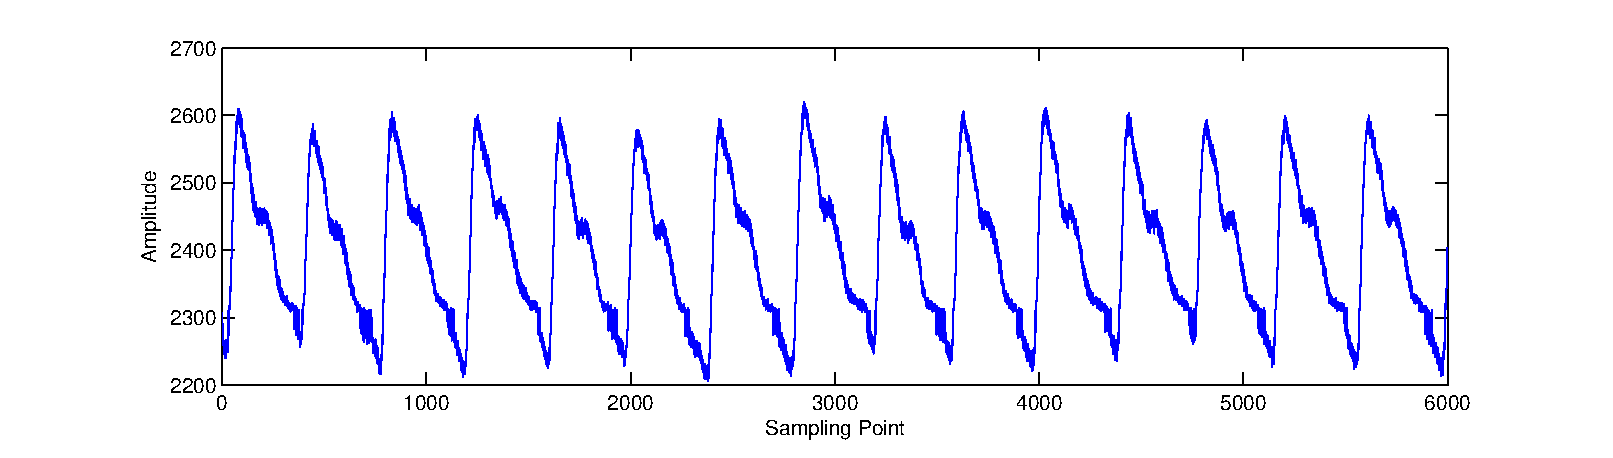
\includegraphics[width=0.7\textwidth]{200g}}\\
    \subfloat[Pulse signal when the pressure is
    250g]{\label{fig:250g}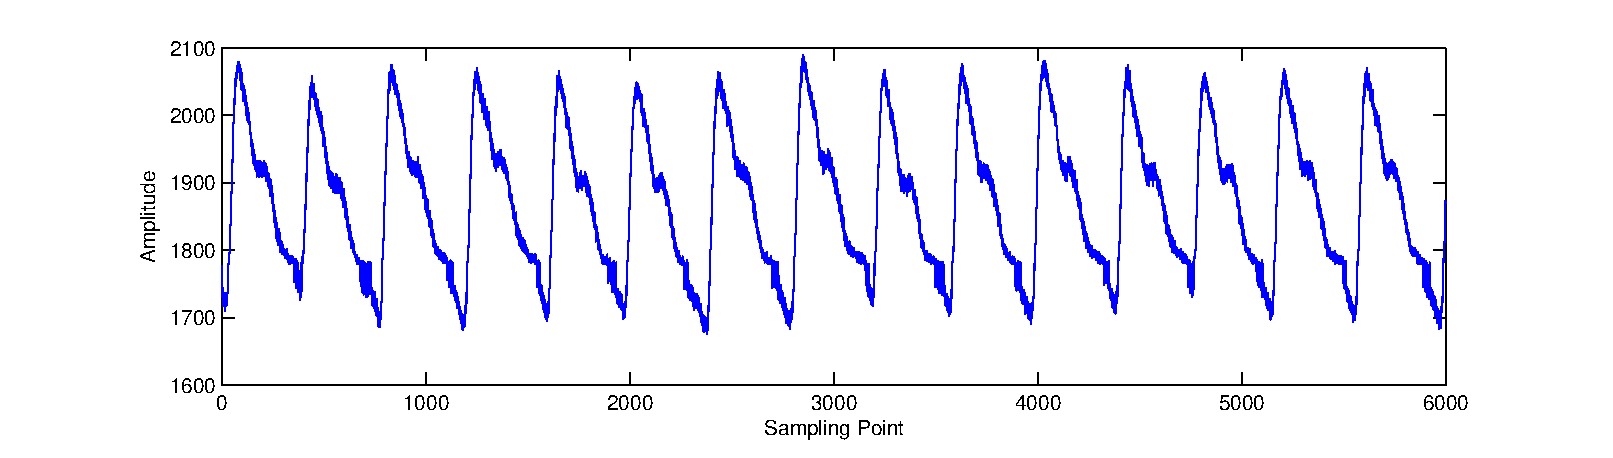
\includegraphics[width=0.7\textwidth]{250g}}\\
    \caption{Pulse signals under three different pressures}
    \label{fig:pressure}
\end{figure}

\section{Pulse database}
After a month of pulse data acquisition, the team has collected 
in total 2247 samples, in which 1565 ones are from physical
examination section and 682 ones are from wards. All the samples are
from Guangdong Hospital of TCM. Table~\ref{tab:database} shows the
main portion of database used in the following chapters. Other sets of
data are either too few in number or information insufficiency. 
The 1565 health examinees are mostly 30 to 40 years old while the rest
682 patients range from 16 to 70 of age. The class of samples results from
western medicine diagnoses provided by the hospital. \todo{再多写一点}
\begin{table}
    \centering
    \begin{tabular}{cc}
        \toprule[1.5pt]
        Disease & Number \\
        \midrule[1pt]
        healthy & 150 \\
        subhealthy & 879 \\
        gastrosia & 28 \\
        nephrosis & 54 \\
        diabetes & 54 \\
        respiratory disease & 33 \\
        angiocardiopathy disease & 35 \\
        endocrine disease & 70 \\
        cardiology & 15 \\
        \bottomrule[1.5pt]
    \end{tabular}
    \caption{Main part of database}
    \label{tab:database}
\end{table}

\section{Summary}
The chapter first introduced four typical sensors: pressure sensor,
photoelectric sensor, microphone, ultrasonic Doppler sensor. The pulse
collecting system in the paper utilized pressure sensor and
photoelectric sensor. In three positions, `Cun', `Guan', `Chi', there
is a probe head which perceives 9-channel photoelectric pulse signals
and one pressure pulse signal. Second, it introduced the advantages and
disadvantages of the system. Third, the paper described the entire collecting
process. The quality of pulse data gathered binds the later
performance of classification. Finally, a pulse database is
established with the pulse information of thousands of people. 
In summary, the automated pulse diagnosis system, to which is widely
payed attention, has important application value. 
Therefore, it significantly makes sense to adopt a exceptional
pulse collecting system to gather accurate pulse information 
and establish a database of rich personal physical information. 

